%% The first command in your LaTeX source must be the \documentclass command.
%%
%% Options:
%% twocolumn : Two column layout.
%% hf: enable header and footer.
\documentclass[
    twocolumn,
% hf,
]{ceurart}

%%
%% One can fix some overfulls
\sloppy

%%
%% Minted listings support
%% Need pygment <http://pygments.org/> <http://pypi.python.org/pypi/Pygments>
\usepackage{minted}
%% auto break lines
\setminted{breaklines=true}

%%
%% end of the preamble, start of the body of the document source.
\begin{document}

%%
%% Rights management information.
%% CC-BY is default license.
    \copyrightyear{2021}
    \copyrightclause{Copyright for this paper by its authors.
    Use permitted under Creative Commons License Attribution 4.0
    International (CC BY 4.0).}

%%
%% This command is for the conference information
    \conference{Proceedings of the 13th Majorov International Conference on Software Engineering
    and Computer Systems,

        December 1--3, 2021, Online \& Saint Petersburg, Russia}

%%
%% The "title" command
    \title{Sparse Representation Approaches for First Stage Retrieval: A Review}

%%
%% The "author" command and its associated commands are used to define
%% the authors and their affiliations.
    \author[1]{Vyacheslav YU. Dobrynin}[%
        email=vidobrynin@itmo.ru
    ]

    \author[1]{Alexey V. Platonov}[%
        email=avplatonov@itmo.ru
    ]

    \address[1]{ITMO University, Kronverksky Pr. 49, bldg. A, Saint-Petersburg, 197101,
        Russian Federation}

%%
%% The abstract is a short summary of the work to be presented in the
%% article.
    \begin{abstract}
        Modern information retrieval models have a two-stage architecture.
        This is due to the requirements - to search for the most relevant documents in a short time.
        For a long time, the attention of researchers was focused on the second stage, the stage
        of ranking a small corpus of documents obtained as a result of the work of the first stage.
        Thanks to neural networks, significant results have been achieved.

        Recently, researchers have begun to pay attention to the first stage, since it is important
        to form as many documents as possible corresponding to a search query for subsequent
        ranking.
        Due to the fact that at this stage it is necessary to work with millions or billions of
        documents, work efficiency is very important.
        An inverted index is very well suited for the task of quickly searching a huge dataset.

        In this paper, we look at modern sparse representation approaches for constructing an
        inverted index.
    \end{abstract}

%%
%% Keywords. The author(s) should pick words that accurately describe
%% the work being presented. Separate the keywords with commas.
    \begin{keywords}
        Information retrieval \sep
        inverted index \sep
        sparse representation \sep
        neural network
    \end{keywords}

%%
%% This command processes the author and affiliation and title
%% information and builds the first part of the formatted document.
    \maketitle


    \section{Introduction}

    Information retrieval predates the web.
    Its evolution was stimulated by various problems associated with providing search and access
    to information sources \cite{manning2008introduction}.
    Applications of this discipline are used to access information in databases of various
    organizations.

    But one of the main engines of progress is web search.
    Now, for most people, this is the main place to find information.

    The requirements for search engines are growing every year, the number of documents is growing,
    and the competition in the market is also high.
    Therefore, it is necessary to improve the quality of the search.

    For a long time, researchers have focused on the ranking stage, but recently, more and more
    papers have appeared that investigate ways to retrieve more relevant documents
    in the first stage.

    Significant results in natural language processing have been achieved through
    the use of embeddings, numerical representations of words or other linguistic entities.
    At the ranking stage, dense embeddings are successfully applied;
    neural networks are used to form them.
    But this approach is computationally ineffective due to the large number of documents that
    need to be worked with at the first stage.
    Therefore, many researchers pay their attention to sparse embeddings.

    In this paper, we will consider some of the currently existing methods for working with sparse
    representations.


    \section{Problem statement}

    \subsection{Modern information retrieval system architecture}

    To combine efficiency and effectiveness when searching for documents in a large corpus, modern
    search engines use multi-stage architectures as shown in the Figure \ref{fig:architecture}.
    \begin{figure}[h]
        \centering
        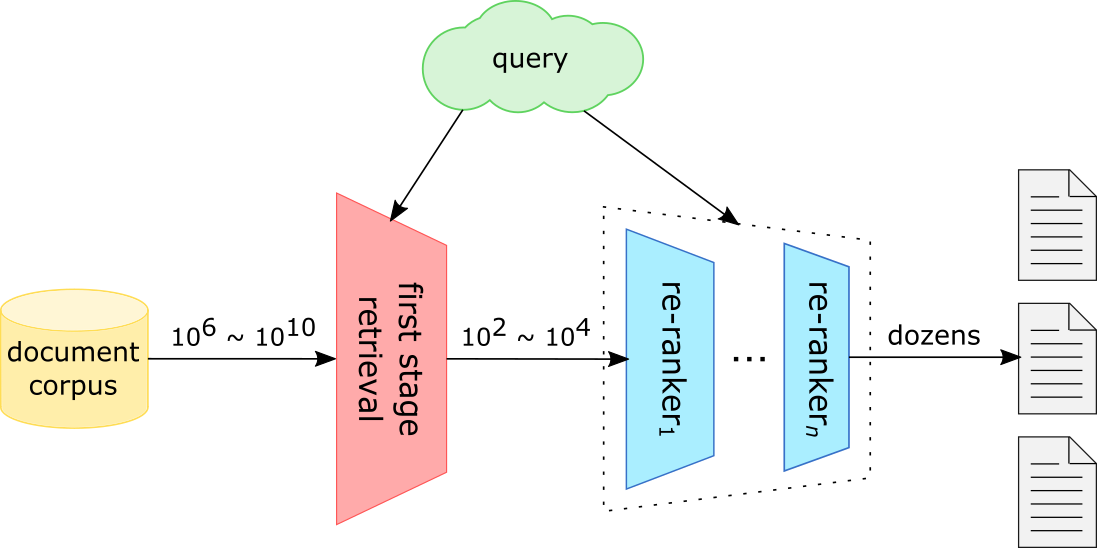
\includegraphics[width=\linewidth]{Architecture.png}
        \caption{The multi-stage architecture of modern information retrieval systems.}
        \label{fig:architecture}
    \end{figure}

    In the first stage, during a search in a large body of documents, the initial set of candidate
    documents is retrieved by using a cheaper ranking model with an inverse index.
    During the second stage, more accurate but slow models are used to reduce the set of
    documents obtained from the first stage and leave the most suitable.
    This approach is widely used in both academic and industrial fields.
    Moreover, it achieved state-of-the-art results.

    \subsection{Problem formalization} \label{problem-formalization}

    Ideally, the goal of the first stage of a search is to retrieve all relevant documents from the
    collection.
    In this regard, when building a model, it is necessary to strive to ensure that it can return
    the most complete set of relevant documents in a short period of time.

    The task at the first stage of extraction is to train the model on the dataset, which will
    evaluate the relevance pairs consisting of a search query and a document.
    The model will give high scores to pairs that have a high relevance and low scores to
    pairs that do not.
    Thus, for any query-document pair (\emph{q}, \emph{d}), model \emph{s}(\emph{q},\emph{d})
    calculates the degree of relevance between the query and the document.
    The scoring function is usually represented as follows:
    \begin{equation}
        s(q,d) = f(\phi(q), \psi(d)),
    \end{equation}
    where \emph{q} \in \emph{X} and \emph{d} \in \emph{Y} are the query and document. $\phi$ and
    $\psi$ are representation functions for map tokens in \emph{X} and \emph{Y} to their
    embeddings $\phi(q)$ and $\psi(d)$.
    To build a model, you need to fulfill the following requirements:
    \begin{itemize}
        \item The document representation function $\psi$ should be independent of the query,
        this allows it to be precomputed and indexed.
        \item The query representation function $\phi$ and scoring function \emph{f} should be as
        efficient as possible, since they are calculated online \cite{SOTA}.
    \end{itemize}

    \subsection{Sparse representation}

    Sparse retrieval methods usually represent each document and each query with sparse vectors,
    where only a small number of dimensions are active.
    The sparse representation has attracted great attention as it connects to the nature of human
    memories and shows better interpretability.

    Besides, sparse representations can be easily integrated into existing inverted indexing
    engines for efficient retrieval.

    Without loss of generality, sparse retrieval methods can be categorized into two classes.
    One is to encode queries and documents still in the symbolic space but employ neural models
    to improve term weighting schemes, namely neural weighting schemes.
    The other is to directly learn sparse representations, i.e., $\phi(q)$ and $\psi(d)$, in
    latent space for queries and documents with neural networks, which we call sparse
    representation learning \cite{SOTA}.


    \section{Models}

    \subsection{SNRM - standalone neural ranking model}

    \begin{figure}[h]
        \centering
        \def\svgwidth{\columnwidth}
        \input{SNRM.pdf_tex}
        \caption{Learning Latent Sparse Representation}
    \end{figure}

    The approach is based on the statement - if you build a neural learning model that meets the
    formal requirements in section \ref{problem-formalization}, then you can build an inverted
    index from the learned representation $\psi(d)$ and receive documents in response to a query
    without a first stage retrieval model.

    Neural network architecture is designed so that parameters can be shared between components
    $\phi(q)$ and $\psi(d)$, which as a result have one semantic space.

    Also, the representations of documents and the query have different levels of sparsity,
    basically for the purpose of greater efficiency, and this is also due to the fact that
    the query is usually much smaller than the document and it is logical to present it as
    representation with fewer elements.

    Therefore, a model is needed in which the representation sparsity is a function
    of the input length.
    Architecture based on Ngram representation learning.
    For each continuous n words in a given document or query, sparse representations are trained,
    which are then aggregated via the average pooling.
    Thus, the document similarity is represented as follows:
    \begin{equation}
        \phi_D(q)=\frac{1}{|d| - n + 1} \sum_{i=1}^{|d| - n + 1} \phi_{ngram}(w_i, w_{i+1}, \cdots, w_{i+n-1})
    \end{equation}
    where $w_1, w_2, \cdots, w_{|d|}$ - terms in document, $\phi_{ngram}$ - learns a sparse representation
    for the given ngram.
    The same function is used for query representation.
    Ngram representation function is a fully-connected feed-forward network that uses a sliding
    window to read the input words and encodes their ngrams.
    Then embeddings are collected for each term \cite{SNRM}.

    \paragraph{Loss Function}
    The loss function for the $i^{th}$ training instance has the following form:
    \begin{equation}
        \mathcal{L}(q_i,d_{i1},d_{i2},y_i) + \lambda\;L_1(\phi_Q(q_i)||\phi_D(d_{i1})||\phi_D(d_{i2}))
    \end{equation}
    where $\mathcal{L}$ - hinge loss \cite{IRNLP}, $q_i$ - query, $d_{i1}$ and $d_{i2}$ - two
    document candidates, $y_i \in \{-1, 1\}$ - label that shows the relevance between the document
    and the query, $\lambda$ - the hyper-parameter to control the sparsity of the learned
    representations, $L_1$ is norm (i.e.
    \begin{math}
        L_1(\vec{\upsilon}) = \sum_{i=1}^{|\vec{\upsilon}|}|\vec{\upsilon}_i|
    \end{math}
    ) and $||$ is concatenation sign.\\\par

    However, SNRM has disadvantage, namely, it loses the interpretability of the original terms,
    which can be significant for industrial systems.

    \subsection{SparTerm}

    \begin{figure}[h]
        \centering
        \def\svgwidth{\columnwidth}
        \input{SparTerm.pdf_tex}
        \caption{General architecture of SparTerm model}
    \end{figure}
    The SparTerm model includes an importance predictor $\mathnormal{F}$ and a gating controller
    $\mathnormal{G}$, it maps the original textual passage \emph{p} to a sparse representation
    $p'$ in the vocabulary.
    This process can be represented as follows:

    \begin{equation}
        \label{eqn:sparterm:mapping-process}
        p' = \mathnormal{F}(p) \odot \mathnormal{G}(p)
    \end{equation}

    $\mathnormal{F}$ generates a dense vector representing the semantic importance of each item
    in the vocabulary. $\mathnormal{G}$ generates a binary gating vector to control which terms
    to appear in the final sparse representation.

    The importance $w_{ij}$ of the token \emph{j} (vocabulary) for token \emph{i} (of the input
    sequence) presented as follows:
    \begin{equation}
        w_{ij}=transform(h_i)^T E_j + b_j \quad j \in {1, ..., |V|}
    \end{equation}
    where \emph{transform(.)} denotes a linear transformation with GeLU
    (Gaussian Error Linear Unit \cite{hendrycks2016gelu}) activation and layer normalization,
    $E_j$ is the BERT input embeddings for token \emph{j} and $b_j$ is the bias term.
    The final representation is then received by the summation of all token-wise importance
    distributions, after applying ReLU to ensure the positivity of term weights:
    \begin{equation}
        \label{eqn:sparterm:importance-predictor}
        w_j=\sum_{i=0}^L ReLU(w_{ij})
    \end{equation}
    where L is the input sequence length.

    \paragraph{Training the importance predictor.}
    There is a set of N training instances $R=\{(q_1, p_{1+}, p_{1-}), ..., (q_N, p_N+, p_N-)\}$,
    each of which contains a query $q_i$, a positive passage $p_{i+}$ and a negative one $p_i-$,
    such that the first passage is more relevant the query than the second one.
    As a result, the loss function has the following form:
    \begin{equation}
        L_{rank}(q_i,p_{i+},p_{i-}) = -log \frac
        {e^{sim(q_i',p_{i+}')}}
        {e^{sim(q_i',p_{i+}')} + e^{sim(q_i',p_{i-}')}}
    \end{equation}
    where $q_i',p_{i+}',p_{i-}'$ is the sparse representation of $q_i,p_{i+},p_{i-}$
    received by Equation (\ref{eqn:sparterm:mapping-process}), \emph{sim} represents a function
    to measure the similarity (e.g. dot product).

    \paragraph{Training the gating controller.}
    Consider a passage-query/summary parallel corpus \emph{C}, which contains passage \emph{p}, the
    cor- responding target text \emph{t}, and the binary bag-of-words vector of \emph{t} (\emph{T}).
    In order to maximize probability values of all terms in vocabulary, binary cross-entropy loss
    is used, which has the following form:
    \begin{equation}
        L_{exp}=-\lambda_1\sum_{j \in \{m|T_m=0\}}log(1-G_j)-\lambda_2\sum_{k \in \{m|T_m=1\}}logG_k
    \end{equation}
    where $\lambda_1$ and $\lambda_2$ are tunable hyper-parameters, first is for terms expected not to be
    expanded, second one is for terms that appear in the target text, and \emph{G} is is the dense
    gating probability distribution for \emph{p} \cite{SparTerm}.\\\par
    Thus, SparTerm provides a function that is used to map the frequency-based and bag-of-words
    representation to a sparse term importance distribution in the whole vocabulary.
    This model also has limitation: since the gating mechanism is learned in advance, this prevents
    the model from learn the optimal sparsification strategy for the ranking task.

    \subsection{SPLADE}

    This approach is based on the SparTerm model, it allows to improve it and get rid
    of the limitation described above.

    \paragraph{Architecture}
    The importance estimation formula Equation (\ref{eqn:sparterm:importance-predictor})
    has been modified by adding a log-saturation effect, in order to prevent the dominance
    of some terms to dominate and naturally ensures sparsity in representations:
    \begin{equation}
        w_j=\sum_{i \in t}log(1+ReLU(w_{ij}))
    \end{equation}

    \paragraph{Loss function}
    The loss function has the following form:
    \begin{equation}
        L_{rank-IBN}=-log
        \frac{
            e^{s(q_i,d_i^+)}
        }{
            e^{s(q_i,d_i^+)} +
            e^{s(q_i,d_i^-)} +
            \sum_j e^{s(q_i,d_{i,j}^-)}
        }
    \end{equation}
    where IBN is in-batch negatives sampling strategy, which is effective for learning first-stage
    rankers \cite{IBN1,IBN2,IBN3}, $q_i$ is query, $d_i^+$ and $d_i^-$ are positive and negative
    documents respectively, ${d_{i,j}^-}$ is set of positive documents from other queries,
    but negative for the current one \cite{SPLADE}.\\\par
    As a result, SPLADE is simple and effective model in information retrieval tasks.

    \subsection{RepBERT}

    For comparison, consider the dense retrieval method called a RepBERT based
    on the popular BERT model.

    \paragraph{Architecture}
    As in BERT\cite{BERT}, the input text is wrapped in [CLS] and [SEP] service marks
    during tokenization:

    \begin{equation}
        Input(text) = [CLS]\;Tokenize(text)\;[SEP]
    \end{equation}

    RepBERT uses an encoder, that finds the averaged value of contextualized vectors for each token
    obtained by passing it to BERT:

    \begin{multline}
        Embed(text)=Encoder(text)=\\
        Average(BERT(Input(text)))
    \end{multline}

    After obtaining the embeddings of queries and documents, RepBERT shares their weights
    to receive relevance scores:

    \begin{equation}
        Rel(query,doc) = Embed(query)^T \cdot Embed(doc)
    \end{equation}

    \paragraph{Training}
    During training, it is necessary to make a embeddings inner product for the relevant
    query-document pairs larger than for the irrelevant ones.
    The model uses the MultiLabelMarginLoss as loss function:
    \begin{multline}
        \mathnormal{L}(q,d_1^+,...,d_m^+,d_{m+1}^-,...,d_n^-) = \\
        \frac{1}{n} \cdot \sum_{1 \leq i \leq m,m < j \leq n}
        max(0, 1 - (Rel(q,d_i^+) - Rel(q,d_j^-)))
    \end{multline}
    where $(q,d_1^+,...,d_m^+,d_{m+1}^-,...,d_n^-)$ is one instance of the input training batch,
    \emph{q} is query, \emph{m} is quantity of relevant documents and \emph{n - m} is quantity
    of irrelevant documents\cite{RepBERT}.\\\par
    The model has a simple architecture in order to improve work efficiency.

% \subsection{UHD-BERT}
% A novel sparse retrieval method empowered by extremely high dimensionality and controllable
%     sparsity. To fully utilize the abundant capacity of representation scheme, proposed bucketed
%     learning, which is a method of learning from the same or different layers of BERT
%     for different aspects or abstraction levels of information.
%     Also introduce and justify choice of WTA model as sparsification model by proving the
%     benefits of reliable representation generation and the ability to control the sparsity
%     at inference time. Show that our model outperforms previous sparse models significantly
%     and delivers competitive performance compared to dense models especially for recall,
%     which is an important measure for a first-stage ranker.


    \section{Evaluation}

    Let's bring the retrieval accuracy for models SparTerm, SPLADE, RepBERT into a pivot table.
    The SNRM model is older and more basic, so it will not be considered.

    To assess the accuracy, the MS MARCO dataset\cite{MS-MARCO} is used.

    The comparison results are shown in the Table \ref{tab:evaluation}.
    Mean Reciprocal Rank (MMR@10) is used as a metric for assessing accuracy.

    \begin{table}[h]
        \caption{The retrieval accuracy (MRR@10) of different approaches. Dataset: MS MARCO.}
        \label{tab:evaluation}
        \begin{tabular}{p{0.4\columnwidth}|p{0.4\columnwidth}}
            \toprule
            Model                   & MRR@10 \\
            \midrule
            SparTerm\cite{SparTerm} & 0.290  \\
            SPLADE\cite{SPLADE}     & 0.322  \\
            RepBERT\cite{RepBERT}   & 0.304  \\
            \bottomrule
        \end{tabular}
    \end{table}


    \section{Conclusion}

    The purpose of this review is to summarize the current research status on sparse representation
    approaches and gain some insights for future development.
    It includes a brief review of existing state-of-the-art sparse retrieval methods, as well as a
    dense retrieval method for an ad-hoc retrieval task.
    A brief description of the approaches is given, illustrations are given, and the necessary
    mathematical equations are outlined.

    At the end, a comparison was made of the approaches considered, from which it can be seen that
    the SPLADE method has the highest accuracy, followed by the compressed RepBERT, but this
    approach are less effective due to the fact that it is based on dense representations.

    The information provided will be used for further research.
    Our focus will be more on sparse representations for the first stage of information retrieval.
    In further works, it is assumed that we have our own stand for researching deep learning
    models in order to form an index in an information retrieval system.

%%
%% Define the bibliography file to be used
    \bibliography{article}

%%
%% If your work has an appendix, this is the place to put it.
    \appendix

\end{document}

%%
%% End of file
